\documentclass[12pt,a4paper]{article} 

\usepackage[spanish]{babel} 
\usepackage[utf8]{inputenc}
\usepackage[numbers,sort&compress]{natbib} %Para la bibliografía
\usepackage{graphicx} %Para incluir figuras
\usepackage{amsfonts}
\usepackage[left=2cm,right=2cm,top=2cm,bottom=2cm]{geometry}
\usepackage{listings}
\usepackage[usenames,dvipsnames]{color}

\lstset{ 
  language=R,
  basicstyle=\scriptsize\ttfamily,
  numbers=left,
  numberstyle=\tiny\color{Blue},
  stepnumber=1,
  numbersep=5pt,
  backgroundcolor=\color{white},
  showstringspaces=false,
  showtabs=false,
  frame=single,
  rulecolor=\color{black},
  tabsize=2,
  captionpos=b,
  breaklines=true,
  breakatwhitespace=false,        
  keywordstyle=\color{RoyalBlue},
  commentstyle=\color{YellowGreen},
  stringstyle=\color{ForestGreen}
}

\title{Matemáticas Computacionales \\ Práctica 1: Gráficas de curvas en R} 
\author{Brenda Esthela Martinez Martinez  1874537}

\begin{document}
\maketitle 

\section{Introducci\'{o}n}\label{sec:intro}

En esta primera práctica realizaremos códigos basicos en R. Se repasaran las curvas en $\mathbb{R}^2$ vistas en primer semestre en la materia de Geometría Analítica. Se graficarán curvas como la recta, parábola, circunferencia, elipse e hipérbola, todo esto con la finalidad de observar y comprobar lo aprendido en Geometría Analítica y para conocer las herramientas de R. Los codigos completos en R se encontraran en \cite{repositorio}.

\section{Linea recta} \label{sec:Linea recta}
\subsection{Definici\'{o}n} \label{subsec:DefLR}
Llamamos línea recta al lugar geométrico de los puntos tales que tomados \emph{dos puntos diferentes cualesquiera $ P_1 (x_1 , y_1) $ y $ P_2 (x_2 , y_2) $ del lugar}, el valor de la pendiente \emph{m} calculado por medio de la formula \ref{eq:Pendiente} 
\begin{equation}
m = \frac{y_1 - y_2}{x_1 - x_2}, x_1 \neq x_2 \label{eq:Pendiente} 
\end{equation}

resulta siempre constante. \cite{geometria}\\ \\

\textbf{ECUACIÓN GENERAL DE LA LINEA RECTA}:
\begin{equation}
y = mx + b \label{eq:pendienteinterseccion}
\end{equation}

\subsection{Ejemplos de gráficas de la línea recta con códigos} \label{subsec:ELR}
%insertar codigo
\begin{table}[htpb]
	\begin{lstlisting}
		#Linea recta 1
		m <- 5 #pendiente
		b <- 0 #interseccion
		
		#Funcion de la linea recta
		f <- function(m, b, x){
		  return(m * x + b)
		  }
		
		x <- seq(1, 10, 0.01)#vector de 1 a 10
		y <- f(m, b, x) #evaluamos
		plot(x, y, type = "l", xlab = "Eje X", ylab = "Eje Y") #graficamos
		abline(h = 10, v = 10) #Linea horizontal en y=10 y linea vertical en x=10
	\end{lstlisting}
	\caption{Primer código en R para gráficar la recta de la figura \ref{fig:recta1}.}
	\label{alg:recta1}
\end{table}
%insertar imagen
\begin{figure}
\centering
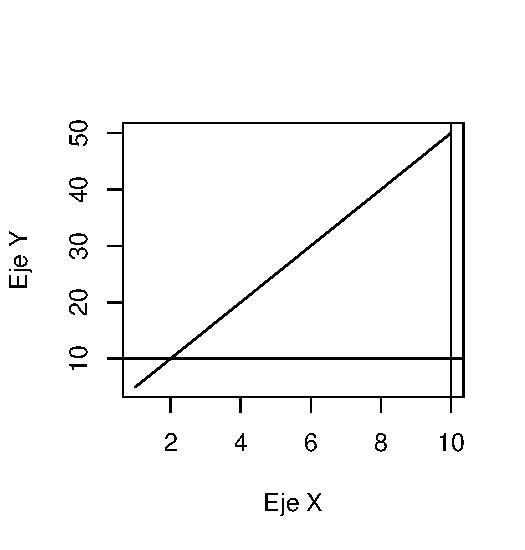
\includegraphics[scale=.8]{LR1}
\caption{Recta 1 con $ m = 5 $}
\label{fig:recta1}
\end{figure}

%insertar codigo
\begin{table}[htpb]
	\begin{lstlisting}
		#Linea recta 1
		m <- 8 #pendiente
		b <- 6 #interseccion
		
		#Funcion de la linea recta
		f <- function(m, b, x){
		  return(m * x + b)
		  }
		
		x <- seq(-5, 12, 0.1)#vector de -5 al 12
		y <- f(m, b, x) #evaluamos
		plot(x, y, type = "l", xlab = "Eje X", ylab = "Eje Y") #graficamos
		abline(h = 0, v = 0) #Linea horizontal en y=0 y linea vertical en x=0
	\end{lstlisting}
	\caption{Segundo código en R para gráficar la recta de la figura \ref{fig:recta2}.}
	\label{alg:recta2}
\end{table}
%insertar imagen
\begin{figure}
\centering
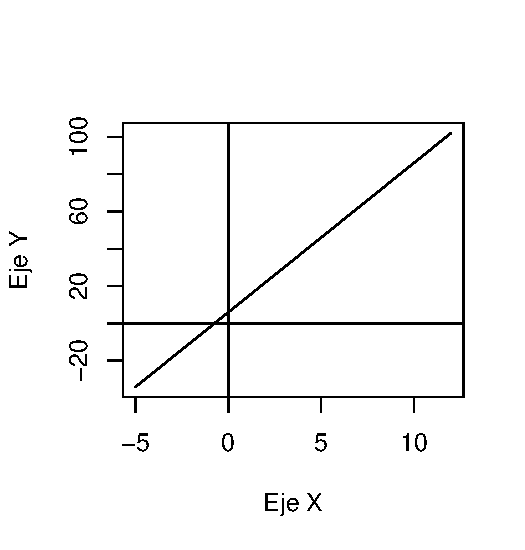
\includegraphics[scale=.8]{LR2}
\caption{Recta 2 con $ m = 8 $}
\label{fig:recta2}
\end{figure}

\section{Parabola} \label{sec:Parabola}

\subsection{Definici\'{o}n} \label{subsec:DefP}
Una \emph{Parábola} es el lugar geométrico de un punto que se mueve en un plano de tal manera que su distancia de una recta fija, situada en el plano, es siempre igual a su distancia de un punto fijo del plano y que no pertenece a la recta. el punto fijo se llama \emph{foco} y la recta fija \emph{directríz} de la parábola. La definicion excluye el caso en el que el foco esta sobre la directriz.\cite{geometria}\\ \\

\textbf{ECUACIÓN GENERAL DE LA PARÁBOLA}

\begin{equation}
y = Ax^2 + Bc + C \label{eq:parabola}
\end{equation}

\subsection{Ejemplos de gráficas de la Parábola con códigos} \label{subsec:EPA}
\begin{table}[htpb]
	\begin{lstlisting}
		#Parabola 1
		g <- function(x){
		  return(3*x^2)
		}
		
		x <- seq(-20, 20, 0.1)#vector de -20 a 20
		y <- g(x)

		plot(x, y, type = "l", xlab = "Eje X", ylab = "Eje Y") #graficamos
		abline(h = 0, v = 0) #lineas en x=0 y y=0
	\end{lstlisting}
	\caption{Primer codigo en R para gráficar la parábola de la figura \ref{fig:parabola1}.}
	\label{alg:par1}
\end{table}

\begin{figure}
\centering
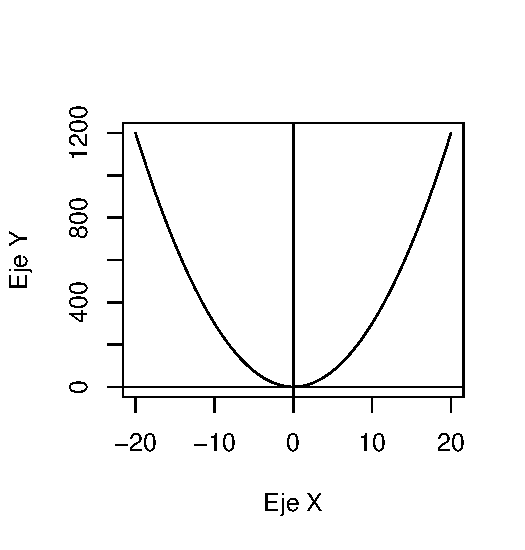
\includegraphics[scale=.8]{PA1}
\caption{Parabola 1: $ 3x^2 $}
\label{fig:parabola1}
\end{figure}

\begin{table}[htpb]
	\begin{lstlisting}
		#Parabola 2
		g <- function(y){
 		 return(y^2)
		}
		
		x <- g(y)
		y <- seq(-10, 10, 0.1)#vector de -20 a 20
		
		plot(x, y, type = "l", xlab = "Eje X", ylab = "Eje Y") #graficamos
		abline(h = 0, v = 0) #lineas en x=0 y y=0
	\end{lstlisting}
	\caption{Segundo codigo en R para gráficar la parábola de la figura \ref{fig:parabola2}.}
	\label{alg:par1}
\end{table}

\begin{figure}
\centering
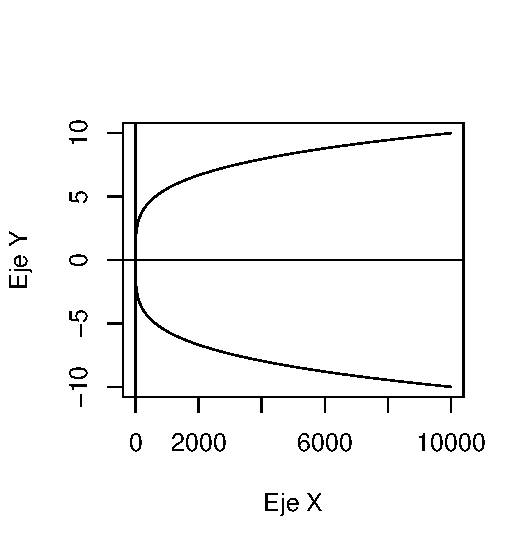
\includegraphics[scale=.8]{PA2}
\caption{Parabola 2: $ y^2 $}
\label{fig:parabola2}
\end{figure}
\newpage
\section{Circunferencia} \label{sec:Circ}
\subsection{Definici\'{o}n} \label{subsec:DefC}
Una \emph{Circunferencia} es el lugar geométrico de un punto que semueve en un plano de tal manera que se conserva siempre a una distancia constante de un punto fijo en ese plano. El punto fijo se llama \emph{centro} de la circunferencia, y la distancia constante se llama \emph{radio}.\cite{geometria}\\ \\

\textbf{ECUACIÓN GENERAL DE LA CIRCUNFERENCIA}
\begin{equation}
(x - h)^2 + (y - k)^2 = r^2, \label{eq:circunferencia}
\end{equation}

\subsection{Ejemplos de gráficas de la Circunferencia con códigos} \label{subsec:ECI}
\begin{table}[htpb]
	\begin{lstlisting}
		#Circunferencia 1
		circunferencia <- function(h, k, r){
 		 if (r >= 0){ # r tiene que ser positivo
   		 if (r == 0){ # si es r = 0, entonces es un punto
 		     plot(x = h, y = k, xlab = "Eje X", ylab = "Eje Y") # grafica del punto
  		  } else{
  		    x <- seq(h - r, h + r, 0.01) # ya que no podemos graficar en todo R^2
  		    ypositiva <- k + sqrt(r^2 - ((x - h)^2)) # parte positiva de la circunferencia
  		    ynegativa <- k - sqrt(r^2 - ((x - h)^2)) # parte negativa de la circunferencia
   		   # graficamos primero la parte positiva
  		    plot(x, ypositiva, type = "l", xlim = c(h - (r + 1), h + (r + 1)), ylim = c(k - (r + 1), k + (r + 1)),
     		      xlab = "Eje X", ylab = "Eje Y")
    		  lines(x, ynegativa, type = "l") # agregamos la parte negativa
    		  abline(h = 0, v = 0) # agregamos los ejes
   		   points(x = h, y = k, col = "red") # dibujamos el centro
   		 }
		  } else{
  		  return(print("El radio no es positivo."))
 		 }
		}
		
		# ejecutamos la funcion
		circunferencia(0, 0, 5)
	\end{lstlisting}
	\caption{Primer codigo en R para gráficar la circunferencia de la figura \ref{fig:circunferencia1}.}
	\label{alg:cir1}
\end{table}

\begin{figure}
\centering
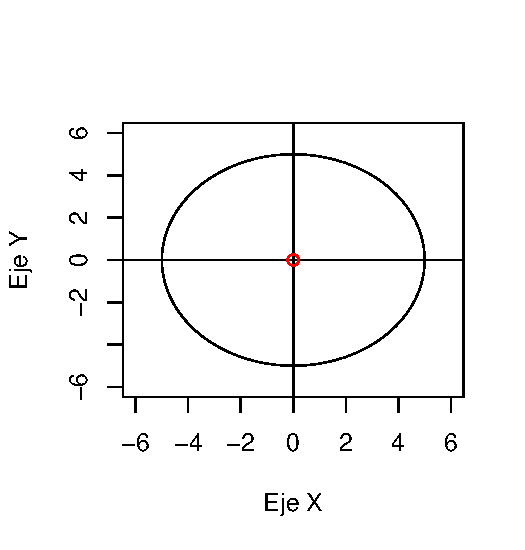
\includegraphics[scale=.8]{CIR1}
\caption{Circunferencia 1: $ x^2+y^2=25 $}
\label{fig:circunferencia1}
\end{figure}

\begin{table}[htpb]
	\begin{lstlisting}
		#Circunferencia 1
		circunferencia <- function(h, k, r){
 		 if (r >= 0){ # r tiene que ser positivo
   		 if (r == 0){ # si es r = 0, entonces es un punto
 		     plot(x = h, y = k, xlab = "Eje X", ylab = "Eje Y") # grafica del punto
  		  } else{
  		    x <- seq(h - r, h + r, 0.01) # ya que no podemos graficar en todo R^2
  		    ypositiva <- k + sqrt(r^2 - ((x - h)^2)) # parte positiva de la circunferencia
  		    ynegativa <- k - sqrt(r^2 - ((x - h)^2)) # parte negativa de la circunferencia
   		   # graficamos primero la parte positiva
  		    plot(x, ypositiva, type = "l", xlim = c(h - (r + 1), h + (r + 1)), ylim = c(k - (r + 1), k + (r + 1)),
     		      xlab = "Eje X", ylab = "Eje Y")
    		  lines(x, ynegativa, type = "l") # agregamos la parte negativa
    		  abline(h = 0, v = 0) # agregamos los ejes
   		   points(x = h, y = k, col = "red") # dibujamos el centro
   		 }
		  } else{
  		  return(print("El radio no es positivo."))
 		 }
		}
		
		# ejecutamos la funcion
		circunferencia(5, 1, 10)
	\end{lstlisting}
	\caption{Segundo codigo en R para gráficar la circunferencia de la figura \ref{fig:circunferencia2}.}
	\label{alg:cir1}
\end{table}

\begin{figure}
\centering
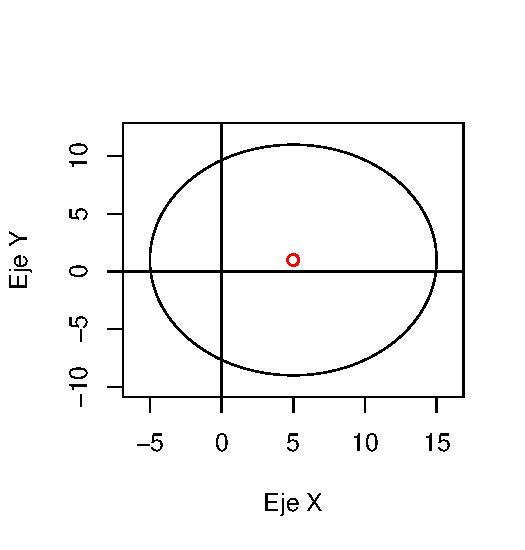
\includegraphics[scale=.8]{CIR2}
\caption{Circunferencia 2: $ (x-5)^2 + (y-1)^2 = 100$}
\label{fig:circunferencia2}
\end{figure}
\newpage
\section{Elipse} \label{sec:Elip}
\subsection{Definici\'{o}n} \label{subsec:DefE}
Una \emph{Elipse} es el lugar geométrico de un punto que se mueve en un plano de tal manera que la suma de sus distancias a dos puntos fijos de ese plano siempre es igual a una constante, mayor que la distancia entre los dos puntos. Los dos puntos fijos se llaman \emph{focos} de la elipse. La definicion de una elipse excluye el caso en que el punto móvil esté sobre el segmento que une los focos.\cite{geometria}\\ \\

\textbf{ECUACIÓN GENERAL DE LA ELIPSE}
\begin{equation}
y = k \pm \sqrt{b^2 - \frac{b^2}{a^2}(x - h)^2} \label{eq:elipse}
\end{equation}

\subsection{Ejemplos de gráficas de la Elipse con códigos} \label{subsec:EEL}
\begin{table}[htpb]
	\begin{lstlisting}
		#Elipse 1
		elipse <- function(h, k, a, b, horizontal){
 		 if (a > b){ # a tiene que ser mayor que b
  		  c <- sqrt(a^2 - b^2) # calculamos c
 		   if (horizontal){ # si es una elipse horizontal
  		    x <- seq(h - a, h + a, 0.01) #definimos el dominio
  		    ypositiva <- k + sqrt((b^2 - (b^2/a^2) * ((x - h)^2))) # parte positiva
  		    ynegativa <- k - sqrt((b^2 - (b^2/a^2) * ((x - h)^2))) # parte negativa
  		    # graficamos primero la parte positiva
   		   plot(x, ypositiva, type = "l", xlim = c(h - (a + 1), h + (a + 1)), ylim = c(k - (b + 1), k + (b + 1)),
   		        xlab = "Eje X", ylab = "Eje Y")
   		   lines(x, ynegativa, type = "l") # agregamos la parte negativa
   		   abline(h = 0, v = 0) # ejes coordenados
   		   points(x = c(h - c, h + c), y = c(k, k), col = "red") # focos
  		  } else{
  		    x <- seq(h - b, h + b, 0.01)
    		  ypositiva <- k + sqrt((a^2 - (a^2/b^2) * ((x - h)^2)))
    		  ynegativa <- k - sqrt((a^2 - (a^2/b^2) * ((x - h)^2)))
    		  plot(x, ypositiva, type = "l", xlim = c(h - (b + 1), h + (b + 1)), ylim = c(k - (a + 1), k + (a + 1)),
   		        xlab = "Eje X", ylab = "Eje Y")
   		   lines(x, ynegativa, type = "l")
   		   abline(h = 0, v = 0)
   		   points(x = c(h, h), y = c(k - c, k + c), col = "red")
   		 }
 		 } else {
  		  return(print("No cumple las condiciones para ser una elipse. (a no es mayor que b)"))
 		 }
		}
	
		elipse(5, 10, 6, 2, TRUE)
	\end{lstlisting}
	\caption{Primer codigo en R para gráficar la elipse de la figura \ref{fig:elipse1}.}
	\label{alg:eli1}
\end{table}

\begin{figure}
\centering
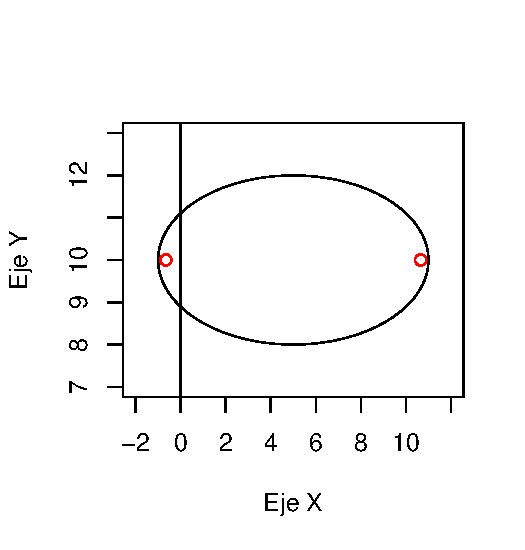
\includegraphics[scale=.8]{ELI1}
\caption{Elipse 1: $ y = 10 \pm \sqrt{2^2 - \frac{2^2}{6^2}(x - 5)^2}  $}
\label{fig:elipse1}
\end{figure}

\begin{table}[htpb]
	\begin{lstlisting}
		#Elipse 2
		elipse <- function(h, k, a, b, horizontal){
 		 if (a > b){ # a tiene que ser mayor que b
  		  c <- sqrt(a^2 - b^2) # calculamos c
 		   if (horizontal){ # si es una elipse horizontal
  		    x <- seq(h - a, h + a, 0.01) #definimos el dominio
  		    ypositiva <- k + sqrt((b^2 - (b^2/a^2) * ((x - h)^2))) # parte positiva
  		    ynegativa <- k - sqrt((b^2 - (b^2/a^2) * ((x - h)^2))) # parte negativa
  		    # graficamos primero la parte positiva
   		   plot(x, ypositiva, type = "l", xlim = c(h - (a + 1), h + (a + 1)), ylim = c(k - (b + 1), k + (b + 1)),
   		        xlab = "Eje X", ylab = "Eje Y")
   		   lines(x, ynegativa, type = "l") # agregamos la parte negativa
   		   abline(h = 0, v = 0) # ejes coordenados
   		   points(x = c(h - c, h + c), y = c(k, k), col = "red") # focos
  		  } else{
  		    x <- seq(h - b, h + b, 0.01)
    		  ypositiva <- k + sqrt((a^2 - (a^2/b^2) * ((x - h)^2)))
    		  ynegativa <- k - sqrt((a^2 - (a^2/b^2) * ((x - h)^2)))
    		  plot(x, ypositiva, type = "l", xlim = c(h - (b + 1), h + (b + 1)), ylim = c(k - (a + 1), k + (a + 1)),
   		        xlab = "Eje X", ylab = "Eje Y")
   		   lines(x, ynegativa, type = "l")
   		   abline(h = 0, v = 0)
   		   points(x = c(h, h), y = c(k - c, k + c), col = "red")
   		 }
 		 } else {
  		  return(print("No cumple las condiciones para ser una elipse. (a no es mayor que b)"))
 		 }
		}
	
		elipse(3, 8, 6, 2, TRUE)
	\end{lstlisting}
	\caption{Segundo codigo en R para gráficar la elipse de la figura \ref{fig:elipse2}.}
	\label{alg:cir1}
\end{table}

\begin{figure}
\centering
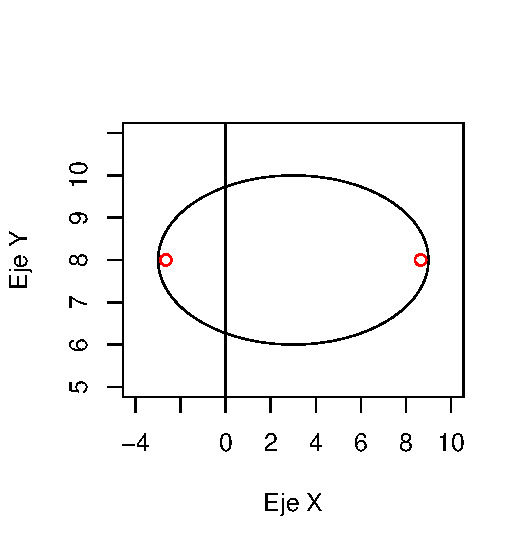
\includegraphics[scale=.8]{ELI2}
\caption{Elipse 2: $ y = 8 \pm \sqrt{2^2 - \frac{2^2}{6^2}(x - 3)^2} $}
\label{fig:elipse2}
\end{figure}

\newpage
\section{Hipérbola} \label{sec:Hiperbola}
\subsection{Definici\'{o}n} \label{subsec:DefH}
Una \emph{Hipérbola} es el lugar geometrico de un punto que se mueve en un plano de tal manera que el valor absoluto de la diferencia de sus distancias a dos puntos fijos en el plano, llamados \emph{focos}, es siempre igual a una cantidad constante, positiva y menor que la distancia entre los focos.\cite{geometria}\\

\textbf{ECUACIÓN GENERAL DE LA HIPÉRBOLA HORIZONTAL}:
\begin{equation}
y = k \pm \sqrt{\frac{b^2}{a^2}(x - h)^2 - b^2}, \label{eq:hiperbolah}
\end{equation}
\textbf{ECUACIÓN GENERAL DE LA HIPÉRBOLA VERTICAL}:
\begin{equation}
x = h \pm \sqrt{\frac{b^2}{a^2}(y - k)^2 - b^2}, \label{eq:hiperobolav}
\end{equation}

\subsection{Ejemplos de gráficas de la Hipérbola con códigos} \label{subsec:EH}

\begin{table}[htpb]
	\begin{lstlisting}
	#Hiperbola 1		
		hiperbola <- function(h, k, a, b, horizontal){
  c <- sqrt(a^2 + b^2) # calculamos c
  if (horizontal){ # hiperbola sobre el eje x
    xizq <- seq(h - (a + 3), h - a, 0.01) # dominio izquierdo
    xder <- seq(h + a, h + (a + 3), 0.01) # dominio derecho
    yizqpositiva <- k + sqrt((b^2/a^2)*((xizq - h)^2) - b^2) 
    yderpositiva <- k + sqrt((b^2/a^2)*((xder - h)^2) - b^2) 
    yizqnegativa <- k - sqrt((b^2/a^2)*((xizq - h)^2) - b^2) 
    ydernegativa <- k - sqrt((b^2/a^2)*((xder - h)^2) - b^2) 
    # graficamos la parte positiva del dominio izquierdo
    plot(xizq, yizqpositiva, type = "l", xlim = c(h - (a + 4), h + (a + 4)), ylim = c(k - (b + 4), k + (b + 4)),
         xlab = "Eje X", ylab = "Eje Y")
    lines(xizq, yizqnegativa, type = "l") # agregamos parte negativa del dominio izquierdo
    lines(xder, ydernegativa, type = "l")
    lines(xder, yderpositiva, type = "l")
    lines(xizq, yizqpositiva, type = "l")
    abline(h = 0, v = 0) # ejes coordenados
    points(x = c(h - (a + c)), y = c(k), col = "red") # focos
    points(x = c(h + (a + c)), y = c(k), col = "red") # focos
  } else{ # hiperbola sobre el eje y
    yizq <- seq(k - (a + 3), k - a, 0.01) # rango inferior
    yder <- seq(k + a, k + (a + 3), 0.01) # rango superior
    xizqpositiva <- h + sqrt((b^2/a^2)*((yizq - k)^2) - b^2) # parte positiva del rango inferior
    xizqnegativa <- h - sqrt((b^2/a^2)*((yizq - k)^2) - b^2) # parte negativa del rango superior
    xderpositiva <- h + sqrt((b^2/a^2)*((yder - k)^2) - b^2) # parte positiva
    xdernegativa <- h - sqrt((b^2/a^2)*((yder - k)^2) - b^2) # parte negativa
    # graficamos
    plot(xizqpositiva, yizq,  type = "l", xlim = c(h - (b + 4), h + (b + 4)), ylim = c(k - (a + 4), k + (a + 4)),
         xlab = "Eje X", ylab = "Eje Y")
    lines(xizqnegativa, yizq, type = "l")
    lines(xizqpositiva, yizq, type = "l")
    lines(xdernegativa, yder, type = "l")
    lines(xderpositiva, yder, type = "l")
    abline(h = 0, v = 0)
    points(x = c(h), y = c(k - (a + c)), col = "red") # focos
    points(x = c(h), y = c(k + (a + c)), col = "red") # focos
  }
}

hiperbola(1, 2, 2, 3, FALSE)
	\end{lstlisting}
	\caption{Primer código en R para gráficar la Hiperbola de ejemplo terminada, que se representa en la figura \ref{fig:hiperbola1}.}
	\label{alg:recta1}
\end{table}
\newpage
\begin{figure}
\centering
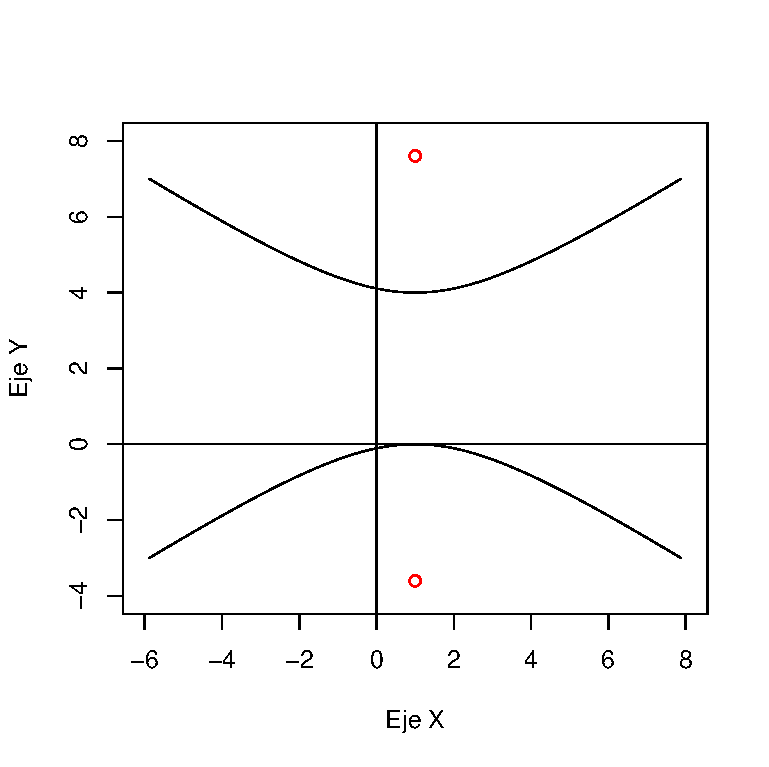
\includegraphics[scale=.8]{HIP1}
\caption{Hiperbola de ejemplo}
\label{fig:hiperbola1}
\end{figure}

%insertar codigo
\begin{table}[htpb]
	\begin{lstlisting}
		#Hiperbola 2		
		#Se utilizan las mismas 28 filas que en el ejemplo 1
		
	hiperbola(0, 1, 1, 5, FALSE)
	\end{lstlisting}
	\caption{Segundo código en R para gráficar la hiperbola de la figura \ref{fig:hiperbola2}.}
	\label{alg:recta2}
\end{table}

\begin{figure}
\centering
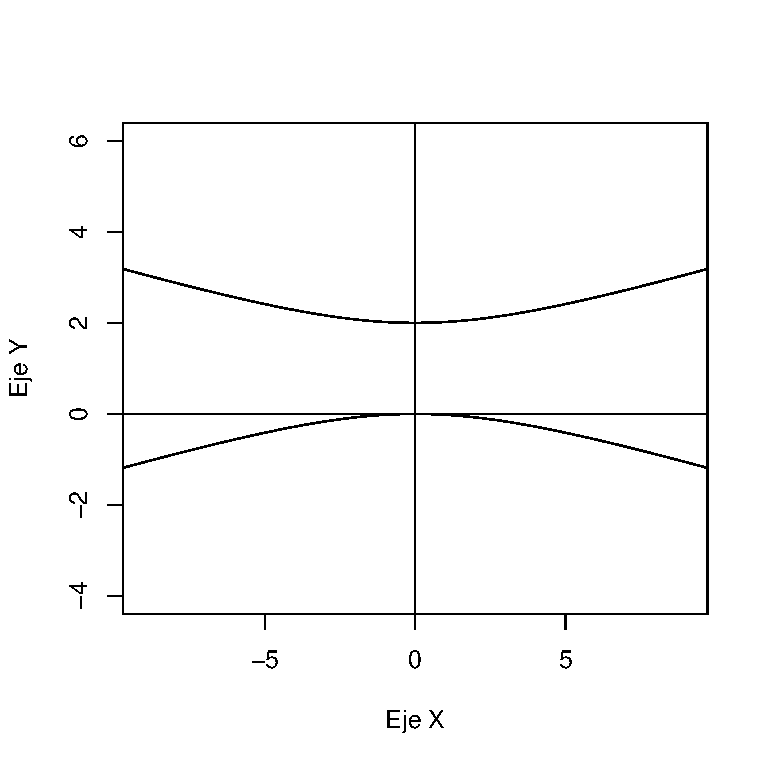
\includegraphics[scale=.8]{HIP2}
\caption{Hiperbola 2}
\label{fig:hiperbola2}
\end{figure}

\begin{table}[htpb]
	\begin{lstlisting}
		#Hiperbola 3		
		#Se utilizan las mismas 28 filas que en el ejemplo 1
		
	hiperbola(1, 2, 2, 3, TRUE)
	\end{lstlisting}
	\caption{Tercer código en R para gráficar la hiperbola de la figura \ref{fig:hiperbola3}.}
	\label{alg:recta2}
\end{table}

\begin{figure}
\centering
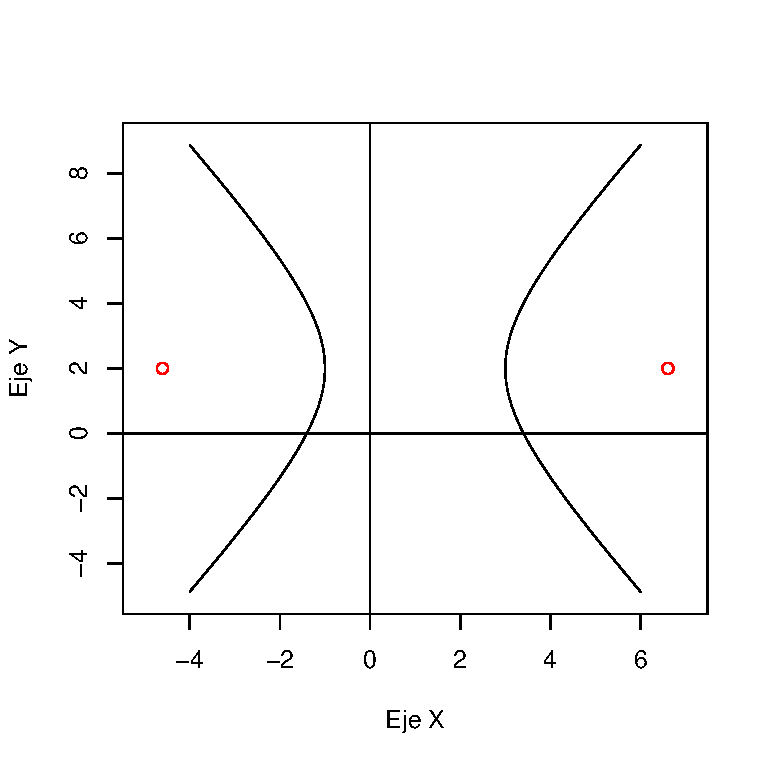
\includegraphics[scale=.8]{HIP3}
\caption{Hiperbola 3}
\label{fig:hiperbola3}
\end{figure}



\newpage
\bibliography{Bibliografia}
\bibliographystyle{plainnat}

\end{document}
